\documentclass{../praktikum-ppt}

\author[Tew \& Haf]{Teosofi Hidayah Agung \\ Hafidz Mulia}
\date{22 Maret 2025}
\title[Alpro 2 - Week 2]{Kompleksitas Algoritma}
\institute[Matematika ITS]{Departemen Matematika\\ Institut Teknologi Sepuluh Nopember}


\begin{document}

{\usebackgroundtemplate{
  \tikz[overlay,remember picture] \node[opacity=0.2, at=(current page.center)]{\includegraphics[width=\paperwidth]{bg_22}};}
\begin{frame}
  \titlepage
\end{frame}
}

\AtBeginSection{
    {\usebackgroundtemplate{
     \tikz[overlay,remember picture] \node[opacity=0.1, at=(current page.center)]{\includegraphics[width=\paperwidth]{code_bg}};}
    \begin{frame}{Daftar isi}
        \tableofcontents[currentsection]
        % \begin{tikzpicture}[overlay, remember picture] 
        %     \node at ([yshift=.5cm]current page.south east) [
        %         anchor = south east, 
        %         ] {
        %     \animategraphics[autoplay,loop,width=0.2\textwidth]{30}{Arisu Dance/Arisu Dance-}{0}{186}
        %     };
        % \end{tikzpicture}
    \end{frame}}
    }

\begin{frame}[fragile]
  \begin{exampleblock}{Warm Up}
    Apakah kedua algoritma berikut menghasilkan output yang sama?
  \end{exampleblock}
  \begin{columns}
    \begin{column}{0.45\textwidth}
      \begin{algorithm}[H]
        \caption{Hmmm}
        \begin{algorithmic}[1]
        \Procedure{Fofo}{$a_1, a_2, \dots, a_n$}
            \State $m \gets 0$
            \For{$i \gets 1$ to $n-1$}
                \For{$j \gets i+1$ to $n$}
                    \If{$|a_i - a_j| > m$}
                        \State $m \gets |a_i - a_j|$
                    \EndIf
                \EndFor
            \EndFor
        \EndProcedure
        \end{algorithmic}
        \end{algorithm}
    \end{column}
    \begin{column}{0.45\textwidth}
      \begin{algorithm}[H]
        \caption{Ermmm}
        \begin{algorithmic}[1]
        \Procedure{Fifi}{$a_1, a_2, \dots, a_n$}
            \State $m_1 \gets a_1$
            \State $m_2 \gets a_1$
            \For{$i \gets 2$ to $n$}
                \If{$a_i < m_1$}
                    \State $m_1 \gets a_i$
                \ElsIf{$a_i > m_2$}
                    \State $m_2 \gets a_i$
                \EndIf
            \EndFor
            \State $m \gets m_2 - m_1$
        \EndProcedure
        \end{algorithmic}
        \end{algorithm}
    \end{column}
  \end{columns}
\end{frame}

\begin{frame}
  Sebuah algoritma haruslah \st{anggaran pendidikan} \textbf{efisien}, artinya:
  \begin{itemize}
    \item Memiliki \textbf{waktu eksekusi} yang cepat.
    \item \textbf{Penggunaan memori} yang optimal.
    \item Ukuran input dapat \textbf{diskalakan} tanpa mempengaruhi kinerja algoritma.
  \end{itemize}
\end{frame}

\section{\textit{Complexity}}
\begin{frame}
  \frametitle{\insertsection}
  \begin{itemize}
    \item \textbf{Kompleksitas waktu} diukur dari jumlah tahapan komputasi yang dilakukan oleh algoritma, biasanya disimbolkan dengan fungsi $T(n)$.
    \item \textbf{Kompleksitas ruang} diukur dari jumlah memori yang digunakan oleh struktur data di algoritma, biasanya disimbolkan dengan fungsi $S(n)$.
  \end{itemize}
  Kompleksitas selalu ditentukan berdasarkan ukuran masukannya.
  \begin{akibat}
    Jika terdapat sebanyak $k$ buah masukan/input, maka kompleksitasnya merupakan fungsi dengan variabel bebas sebanyak $k$. ($F(n_1, n_2, \ldots, n_k)$)
  \end{akibat}
\end{frame}

\begin{frame}
  \frametitle{\insertsection}
  \begin{contoh}
    \textit{Method} penjumlahan dan perkalian matriks bergantung pada ukuran matriks yang diinputkan.
  \end{contoh}
  \begin{contoh}
    Menghitung FPB atau KPK dari dua bilangan bergantung pada kedua bilangan tersebut.
  \end{contoh}
  \begin{contoh}
    Mencari nilai terbesar (maksimum) dari sebuah array bergantung pada panjang array.
  \end{contoh}
\end{frame}

\subsection{Kompleksitas Waktu}
\begin{frame}
  \frametitle{\insertsection}
  \framesubtitle{\insertsubsection}
  \begin{block}{Kompleksitas Waktu}
    \begin{itemize}
      \item \textbf{Worst Case} $T_{max}(n):=$ Kompleksitas waktu terburuk yang mungkin terjadi.
      \item \textbf{Best Case} $T_{min}(n):=$ Kompleksitas waktu terbaik yang mungkin terjadi.
      \item \textbf{Average Case} $T_{avg}(n):=$ Kompleksitas waktu rata-rata yang mungkin terjadi.
    \end{itemize}
  \end{block}
\end{frame}
\begin{frame}
  \frametitle{\insertsection}
  \framesubtitle{\insertsubsection}
  \begin{block}{Kompleksitas Waktu}
  Biasanya hitungan kompleksitas waktu meliputi:
  \begin{itemize}
    \item Operasi baca/tulis $\quad$ \textcolor{green!50!black}{(\texttt{input a, print a})}
    \item Operasi aritmatika $\quad$ \textcolor{green!50!black}{(\texttt{b + c, m * n})}
    \item Operasi perbandingan $\quad$ \textcolor{green!50!black}{(\texttt{a < b, x == y})}
    \item Operasi \textit{assignment} $\quad$ \textcolor{green!50!black}{(\texttt{a $\leftarrow$ b, x $\leftarrow$ 5})}
    \item dll.
  \end{itemize}
  \end{block}
\end{frame}

\begin{frame}
  \frametitle{\insertsection}
  \framesubtitle{\insertsubsection}
  \begin{itemize}
    \item \textbf{Algoritma pencarian (searching)} \\
    Operasi khas: operasi perbandingan elemen larik.
    
    \item \textbf{Algoritma pengurutan (sorting)} \\
    Operasi khas: operasi perbandingan elemen dan operasi pertukaran elemen.
    
    \item \textbf{Algoritma perkalian dua buah matriks \( AB = C \)} \\
    Operasi khas: operasi perkalian dan penjumlahan.
\end{itemize}
\end{frame}

\begin{frame}
  \frametitle{\insertsection}
  \framesubtitle{\insertsubsection}
  \begin{algorithm}[H]
    \caption{Cari Maksimum}
    \begin{algorithmic}[1]
    \Procedure{Max}{$a_1, a_2, \dots, a_n$} \Comment{Input: Array integer}
        \State $max \gets a_1$ \Comment{Inisialisasi dengan elemen pertama}
        \For{$i \gets 2$ to $n$}
            \If{$max < a_i$} \State $max \gets a_i$
            \EndIf
        \EndFor
        \State \Return $max$ \Comment{Nilai maksimum dalam array}
    \EndProcedure
    \end{algorithmic}
    \end{algorithm}
    \onslide<2->{\begin{exampleblock}{}
        Operasi dasarnya adalah perbandingan elemen ($max < a_1$) yang dilakukan sebanyak $n-1$ kali. Kompleksitas waktu: $T(n)=n-1$
    \end{exampleblock}}
\end{frame}

\begin{frame}
  \frametitle{\insertsection}
  \framesubtitle{\insertsubsection}
  \begin{algorithm}[H]
    \caption{Perhitungan dengan Nested Loop dan Pembagian}
    \begin{algorithmic}[1]
    \State \textbf{Input}: $n$
    \State $j \gets n$, $x \gets 1$
    \While{$j \geq 1$}
        \For{$i \gets 1$ to $j$} $x \gets x \times i$
        \EndFor
        \State $j \gets j \div 2$
    \EndWhile
    \State jumlah $\gets x$
    \end{algorithmic}
  \end{algorithm}
  \onslide<2->{\begin{exampleblock}{}
    Kompleksitas waktu: $T(n)=n\left(2-\dfrac{1}{2^{n-1}}\right)$
  \end{exampleblock}}
\end{frame}

\subsection{Kompleksitas Ruang}
\begin{frame}
  \frametitle{\insertsection}
  \framesubtitle{\insertsubsection}
  \begin{block}{Kompleksitas Ruang}
    \begin{itemize}
      \item \textbf{Worst Case} $S_{max}(n):=$ Kompleksitas ruang terburuk yang mungkin terjadi.
      \item \textbf{Best Case} $S_{min}(n):=$ Kompleksitas ruang terbaik yang mungkin terjadi.
      \item \textbf{Average Case} $S_{avg}(n):=$ Kompleksitas ruang rata-rata yang mungkin terjadi.
    \end{itemize}
  \end{block}
  \begin{alertblock}{Fakta saat ini}
     Kompleksitas ruang tidak akan dibahas lebih jauh karena pada dasarnya solusi untuk permasalahan \textit{storage} lebih mudah diatasi daripada \textit{running time}. 
  \end{alertblock}
\end{frame}

\begin{frame}[fragile]
  \frametitle{\insertsection}
  \framesubtitle{\insertsubsection}
  Analisa kompleksitas ruang biasanya digunakan untuk fungsi tipe rekursif.
  \begin{contoh}
    Space complexity: $S(n)=n$
  \end{contoh}
  \begin{lstlisting}[caption={Jumlahan $n$},captionpos=b]
  int sum(int n){
    if (n <= 0)return 0;
    return n + add (n-1);
  }
  \end{lstlisting}
  Program akan menyimpan $n$ nilai memori sebelum fungsi berakhir.
\end{frame}

\begin{frame}[fragile]
  \frametitle{\insertsection}
  \framesubtitle{\insertsubsection}
  \begin{contoh}
    Space complexity: $S(n)=1$
  \end{contoh}
  \begin{lstlisting}[caption={Faktorial},captionpos=b]
  int addSequence(int n){
    int sum = 0;
    for (int i = 0; i < n; i++){
        sum += pairSum(i, i+1);
    }
    return sum;
  }
  int pairSum(int x, int y){
    return x + y;
  }
  \end{lstlisting}
  Program hanya menyimpan satu nilai memori selama eksekusi. (tidak ter-\textit{stack})
\end{frame}

\begin{frame}[fragile]
  \frametitle{\insertsection}
  \framesubtitle{\insertsubsection}
  \begin{contoh}
    Space complexity: $S(n)=2^n$
  \end{contoh}
  \begin{lstlisting}[caption={Fibonacci},captionpos=b]
  int fib(int n){
    if (n <= 1)return n;
    return fib (n-1) + fib (n-2);
  }
  \end{lstlisting}
  Program memiliki 2 cabang setiap pemanggilan fungsi, sehingga memori yang digunakan akan berlipat dua setiap pemanggilan.
\end{frame}


\section{Big-O}
\begin{frame}
  \frametitle{\insertsection}
  \begin{quote}
    \centering
    \textbf{``Hope for the best, \underline{prepare for the worst}.''}
  \end{quote}
  \begin{masalah}
    Dalam pemograman dan algoritma, $T_{max}(n)$ seringkali menjadi fokus utama daripada karena meminimalisir kemungkinan terburuk lebih penting daripada memaksimalkan kemungkinan terbaik.\\

    Namun tidak semua program memiliki kompleksitas waktu yang dapat dideterminasi. Sehingga diperlukan pendekatan lain untuk mendefinisikan kompleksitas waktu secara umum.
  \end{masalah}
\end{frame}

\begin{frame}
  \frametitle{\insertsection}
  \begin{definisi}[Big-O]
    Misalkan $f(n)$ dan $g(n)$ adalah dua fungsi. Kita mengatakan bahwa $f(n)$ adalah $\bigO(g(n))$ jika dan hanya jika terdapat konstanta positif $C$ dan $n_0$ sedemikian sehingga
\[
C \cdot g(n) > f(n)
\]
untuk semua $n > n_0$. Biasanya disimbolkan sebagai $f(n) = \bigO(g(n))$ atau $f(n) \in \bigO(g(n))$.
  \end{definisi}
  Untuk alasan praktikal, nantinya kita akan memilih fungsi $g(n)$ sekecil mungkin agar $\bigO(g(n))$ memiliki makna.
\end{frame}

\begin{frame}
  \frametitle{\insertsection}
  \begin{contoh}
    \begin{itemize}
      \item $f(n) = 2n^2 + 3n + 1$ dan $g(n) = n^2$ \\
      Karena $2n^2 + 3n + 1 \leq 2n^2 + 3n^2 + n^2 = 6n^2$ untuk $n > 1$\\
      atau $2n^2 + 3n + 1 \leq n^2 + n^2 + n^2 = 3n^2$ untuk $n > 34$, maka $f(n) \in \bigO(n^2)$.
      \item $f(n) = \ln(x+4)$ dan $g(n) = \log n$ \\
      Karena $\ln(x+4) \leq 6\log n$ untuk $n > 2$, maka $f(n) \in \bigO(\log n)$.
      \item $T(n)=6\cdot 2^n+2n^2$ dan $g(n)=2^n$ \\
      Karena $6\cdot 2^n+2n^2 \leq 6\cdot 2^n+2\cdot 2^n = 8\cdot 2^n$ untuk $n > 1$ ($C=8$, $n_0=1$), maka $T(n) \in \bigO(2^n)$.
    \end{itemize}
  \end{contoh}
\end{frame}

\begin{frame}
  \frametitle{\insertsection}
  \begin{teorema}
    untuk $n$ yang cukup besar, berlaku
    \[1<\log n<n^r<a^n<n!<n^n\]
    untuk $r\geq 1$ dan $a>1$.
  \end{teorema}
  \begin{center}
    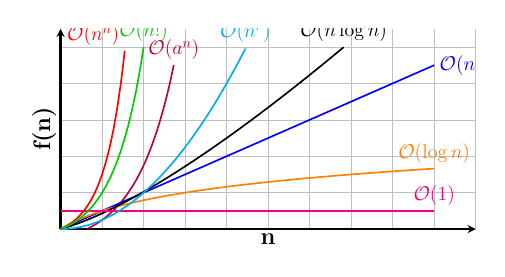
\begin{tikzpicture}[scale=0.5]
      \begin{axis}[
        grid = major,
        clip = true,
        ticks = none,
        width=1.0\textwidth,
        height=0.55\textwidth,
        every axis plot/.append style={very thick},
        axis line style = ultra thick,
        clip mode=individual,
        restrict y to domain=0:10,
        restrict x to domain=1:10,
        axis x line = left,
        axis y line = left,
        domain = 1:10,
        xmin = 1,
        xmax = 11,
        ymin = 0,
        ymax = 11,
        xlabel = n,
        ylabel = f(n),
        xlabel style = {at={(axis description cs:0.5,-0.1)},anchor=south},
        ylabel style = {at={(axis description cs:-0.08,0.5)},anchor=north},
        label style = {font=\LARGE\bf},
      ]
    \addplot [
        samples=100, 
        color=purple,
    ]
    {1/2*3^(x-1)-1}node[above,pos=1,style={font=\Large}]{$\mathcal{O}(a^n)$};
    \addplot [
        samples=100, 
        color=blue,
    ]
    {x-1}node[right,pos=1,style={font=\Large}]{$\mathcal{O}(n)$};
    \addplot [
        samples=100, 
        color=orange,
    ]
    {log2 x}node[above,pos=1,style={font=\Large}]{$\mathcal{O}(\log n)$};
    \addplot [
        samples=100, 
        color=black,
    ]
    {x*(ln(x)/ln(5))}node[above,pos=1,style={font=\Large}]{$\mathcal{O}(n\log n)$};
    \addplot [
        samples=100, 
        color=magenta,
    ]
    {1}node[above,pos=1,style={font=\Large}]{$\mathcal{O}(1)$};
    \addplot [
        samples=100, 
        color=cyan,
    ]
    {1/2*(x-1)^(2)}node[above,pos=1,style={font=\Large}]{$\mathcal{O}(n^r)$};

    \addplot [
        samples=100, 
        color=red,
    ]
    {x^x-1}node[above left,pos=1,style={font=\Large}]{$\mathcal{O}(n^n)$};
    
    %Creates stair-step like plot

    \addplot [
      samples=100,
      color=green!80!black, 
    ] {2*sqrt(2*pi)*(x+1)^(x+0.5)*exp(-x-1)*exp(1/(12*x+12))-2} node[above,pos=1,style={font=\Large}]{$\mathcal{O}(n!)$};
    
    \end{axis}
    \end{tikzpicture}
  \end{center}
\end{frame}

\begin{frame}
  \frametitle{\insertsection}
  \begin{teorema}
    Misalkan \( T_1(n) = O(f(n)) \) dan \( T_2(n) = O(g(n)) \), maka
    \begin{itemize}
        \item \( T_1(n) + T_2(n) = O(f(n)) + O(g(n)) = O(\max(f(n), g(n))) \)
        \item \( T_1(n)T_2(n) = O(f(n)) O(g(n)) = O(f(n) g(n)) \)
        \item \( O(cf(n)) = O(f(n)) \), \( c \) adalah konstanta
        \item \( f(n) = O(f(n)) \)
    \end{itemize}
  \end{teorema}
\end{frame}

\begin{frame}
  \frametitle{\insertsection}
  \begin{alertblock}{Bentuk Sederhana}
    Ingat, di dalam notasi Big-Oh tidak ada koefisien atau suku-suku lainnya, hanya berisi fungsi-fungsi standard seperti 
    \( 1, n^2, n^3, \dots, \log n, n \log n, 2^n, n! \), dan sebagainya. Contoh:
    \begin{itemize}
      \item \( O(2n) \) tidak standard, seharusnya \( O(n) \)
      \item \( O(\log(n^2)) \) tidak standard, seharusnya \( O(\log n) \)
      \item \( O\left(\dfrac{n^2}{2}\right) \) tidak standard, seharusnya \( O(n^2) \)
      \item \( O((n - 1)!) \) tidak standard, seharusnya \( O(n!) \)
  \end{itemize}
  \end{alertblock}
\end{frame}

\section{Latihan}
\begin{frame}
  \begin{latihan}
  Tunjukkan/buktikan pernyataan berikut:
  \begin{itemize}
    \item $1+2+3+\cdots+n = \bigO(n^2) $
    \item $n! = \bigO(n^n) $
    \item $\log n! = \bigO(n\log n)$
    \item $2^n = \bigO(3^n)$
    \item $(n+1)\log(n^3+2)+4n^2\in\bigO(n^2)$
  \end{itemize}
  \end{latihan}
\end{frame}

\begin{frame}[fragile]
  \begin{latihan}
    Jawablah pertanyaan dibawah ini yang mengacu pada algoritma dibawahnya
    \begin{itemize}
      \item Apa yang dilakukan algoritma berikut?
      \item Berapakah kompleksitas waktu dari algoritma berikut? Tuliskan jawaban dalam notasi Big-O.
      \item Coba ubahlah algoritma tersebut agar lebih efisien terhadap kompleksitas waktu.
    \end{itemize}
  \end{latihan}
  \begin{lstlisting}
    public static int solution(int n) {
        int solutions = 0;
        for (int a = 0; a <= n; a++) 
            for (int b = 0; b <= n; b++) 
                for (int c = 0; c <= n; c++) 
                    if (a + b + c == n) solutions++;

        return solutions;
    }
  \end{lstlisting}
\end{frame}

\end{document}